\documentclass[]{amsart}
\usepackage[T1]{fontenc}
\usepackage[latin1]{inputenc}
\usepackage{amsfonts,verbatim}
\usepackage{amssymb,amsthm}
\usepackage{amsmath}
\usepackage{graphicx}
\usepackage{psfrag}

\usepackage{graphicx}
\author{Daniel Appel\"{o}}
\title{Method of Manufactured Solution or Twilight Zone Forcing}
\begin{document}
\maketitle
Say that we are interested in finding a discrete approximation, $v$, to the solution of the initial-boundary-value-problem 
\begin{align}
&u_{tt}=u_{xx}+f, \ \ t > 0,\, x\in[0,1], \label{pde}\\
& u(x,0) = u_0(x),\label{ic}\\
& \alpha_0 u(0,t) +\alpha_1 u_x(0,t) = u_l(t), \label{bc0}\\ 
& \beta_0 u(1,t) +\beta_1 u_x(1,t) = u_r(t), \label{bc1}
\end{align}
by implementing some numerical method on a computer. How can we convince ourselves (and the instructor or TA) that the code  is implementing the numerical method and thus approximating the ivbp correctly? 

Assume that the numerical method has an error that converges to zero with some discretization parameter $h$ (usually the grid spacing) as $\mathcal{O}(h^r)$. Then a good test is to measure the error 
\[
\epsilon_p(t)= \left( 
\int_0^1 |u-v|^p \,dx
\right)^{\frac{1}{p}},
\]
for some different values of $h$ and make sure that $\epsilon_p \sim \mathcal{O}(h^r)$, as advertised. The crux of the matter is that the computation of $\epsilon_p$ require the knowledge of $u$, which we don't know! 

This is where the method of manufactured solution comes in. If we want the solution to be, say,  
\begin{equation}\label{mms}
u(x,t) = \sin(\omega (t+t_0) -k x),
\end{equation}
how should we adjust (\ref{pde})-(\ref{bc1}) so that (\ref{mms}) hold? The answer is simple, we just have to choose the forcing, initial- and boundary-conditions we get by plugging in (\ref{mms}). For example, with $u$ as above, we would get:
\begin{align*}
& f(x,t)=(k^2-\omega^2) \sin(\omega (t+t_0) -k x),\\ 
& u(x,0) = \sin(\omega (t+t_0) -k x),\\
& u_l(t) =\alpha_0 \sin(\omega (t+t_0)) - \alpha_1 k \cos(\omega (t+t_0)),\\ 
& u_r(t) = \beta_0 \sin(\omega (t+t_0) -k) -\beta_1 k \cos(\omega (t+t_0)-k). 
\end{align*}
\subsection*{Strategy for easy implementation and debugging}
The strategy is simple: 1. Split the numerical method into smaller subproblems. 2. Implement each subproblem in a subroutine and {\bf test} it separately. 3. Assemble the subroutines into a program and test it again. If the results are really important you should also: 4. Ask someone else to write a separate program (solving the same problem) and compare the results. This may seem tedious but in the end it will save you time. Once you get it right with the manufactured solution you can change the forcing etc. back to whatever you wanted to use in the first place. 

For example, for the problem (\ref{pde})-(\ref{bc1}) we need subroutines that:
\begin{enumerate}
\item Compute initial data. 
\item Compute the forcing $f(x,y)$.
\item Given the solution in the interior, compute and assign boundary conditions.
\item Given the solution everywhere, compute an approximation to $u_{xx}$.
\item Advance the solution in time.
\end{enumerate}
Fortunately, now that we know the exact solution for a particular forcing, initial- and boundary-conditions we can test every subroutine in the code separately (rather than writing the code from scratch and compute the error at the end). 

Again, you might think that, as there is only 5 subroutines, it is unnecessary to test them separately, {\bf this is a serious misunderstanding!} As those of you who have experience in programming know, getting 5 subroutines to work simultaneously is not 5 times harder it is $m^5$ times harder (here $m$ is a number that is reduced as you get more experienced but for most human beings it never becomes smaller then 2). 

\begin{figure}[t]
  \begin{center}
 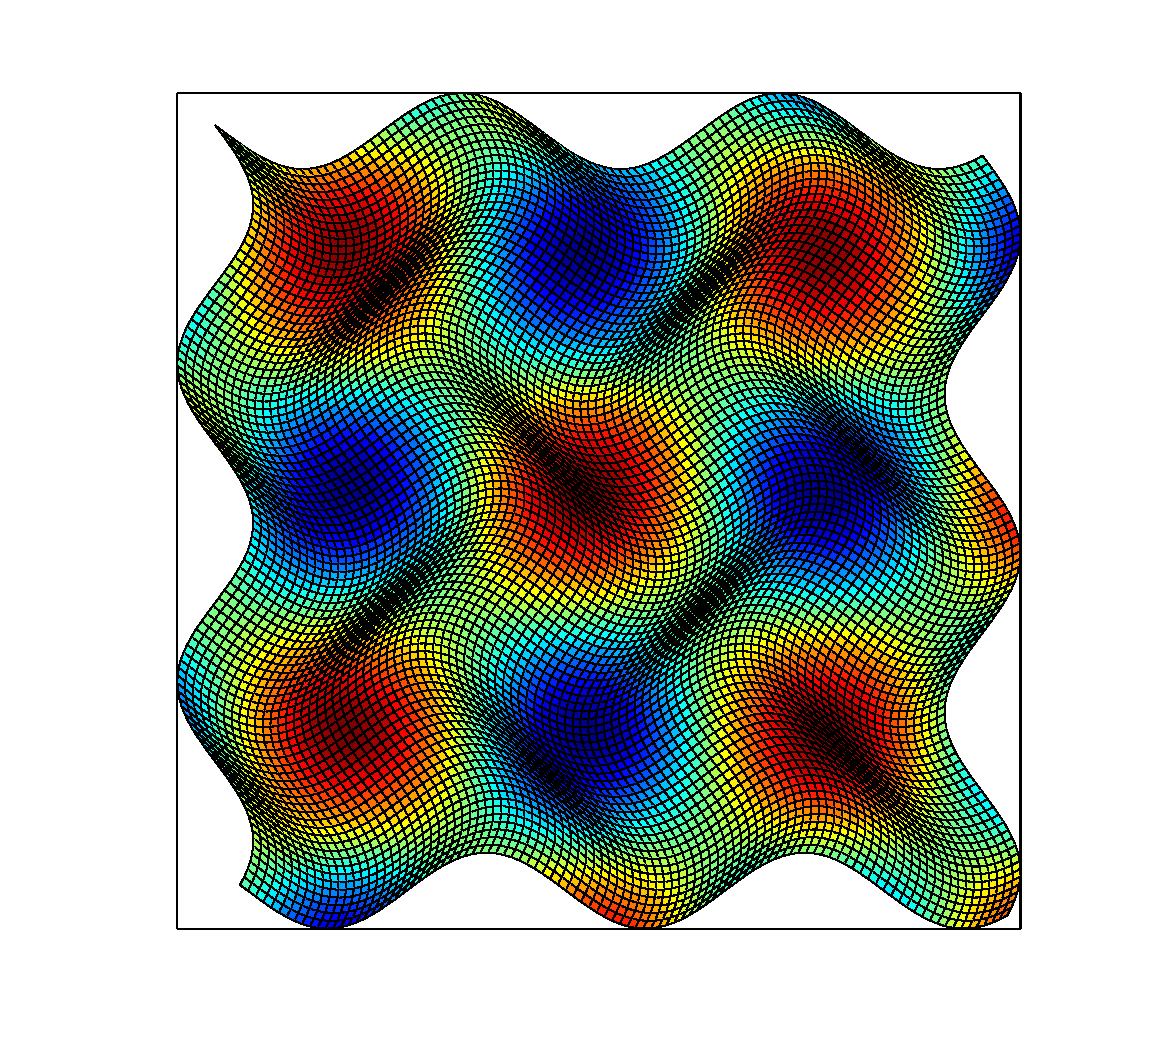
\includegraphics[width=0.75\textwidth]{mmsgrid}
    \caption{Solution using method of manufactured solution.\label{fig:mms}}
  \end{center}
\end{figure}
If your thesis work requires that you develop code then I suggest you use this course to build a library of routines of different exact solutions (and their derivatives w.r.t. time and space). 

Two solutions that are commonly used are the trigonometric solution
\[
u(x,y,z,t)= \sin(\omega (t+t_0) -k_x x) \sin( k_y y)\sin(k_z z),
\]
and the polynomial solution
\[
u(x,y,z,t)= \left(\sum a_i t^i \right) \left(\sum b_j x^j \right)\left(\sum c_k y^k \right)\left(\sum d_l x^l \right).
\]
The polynomial solution is very useful for testing separate routines as the approximated solution will be \emph{exact} if the degree of the polynomials are low enough (a second order method is often exact for first order polynomials).  
The trigonometric solution, being bounded by 1, is well suited if you need to monitor the error over a long time interval. This can be useful if you need to understand the mechanisms behind some numerical instability. 

I cannot stress enough how useful it is to use the method of manufactured solution\footnote{I recently wrote a solver for the elastic wave equation on a general metric in $(3+1)$ dimensions, where there are 127 $u_{xx}$-type terms to account for. The subroutine approximating the derivatives ended up being more than 44000 lines and without the exact solution I would never have got it right.}, if you start using it now it will save you {\bf countless hours} once you start implementing more complicated algorithms.




\subsection*{Why Twilight Zone?}
The expression \emph{Twilight Zone solution} or \emph{Twilight Zone forcing} comes from the similarity between the trigonometric solution (see Figure \ref{fig:mms}) and the spiral in the TV-show the Twilight Zone. The expression was coined by David Brown at Los Alamos sometimes in the 80s or 90s.   
\end{document} 
